\uuid{jgqL}
\exo7id{7166}
\titre{exo7 7166}
\auteur{megy}
\organisation{exo7}
\datecreate{2017-07-08}
\isIndication{false}
\isCorrection{true}
\chapitre{Nombres complexes}
\sousChapitre{Géométrie}

\contenu{
\texte{
% parallélogramme de Varignon, minimisation de périmètre
Soit $M_1M_2M_3M_4$ un parallélogramme direct du plan, de centre $O$, et $A$ un point quelconque du plan. On considère $B$ le symétrique de $A$ par rapport à $M_1$, $C$ le symétrique de $B$ par rapport à $M_2$, $D$ le symétrique de $C$ par rapport à $M_3$ et $E$ le symétrique de $D$ par rapport à $M_4$.
\begin{center}
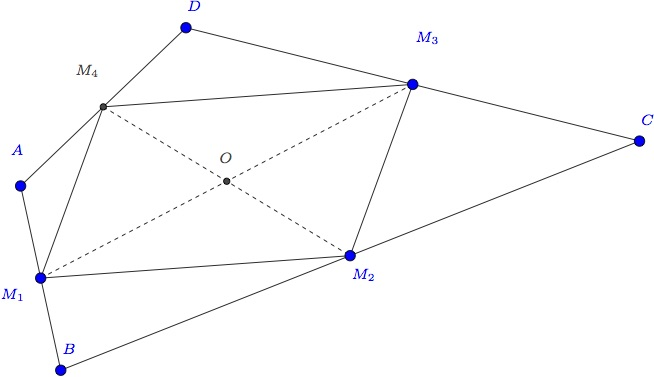
\includegraphics{../images/img007166-1}
\end{center}
}
\begin{enumerate}
    \item \question{Montrer que $E=A$.}
\reponse{Le point $E$ est l'image de $A$ par la composée des quatre symétries centrales de centre $M_1$,  ... $M_4$. Montrons que cette composée est l'identité. Par le cours, le composée de ces quatre rotations est une translation. Il suffit alors de tester un point particulier pour vérifier que c'est l'identité. Si $A=M_1$ par exemple, on voit que $A=E$ en utilisant le théorème de Thalès.}
    \item \question{Montrer que si $z$ et $z'$ sont deux complexes, alors $|z+z'|+|z-z'|\geq 2|z|$.}
\reponse{On a $2z = (z+z')+(z-z')$, d'où par inégalité triangulaire $2|z| \leq |z+z'|+|z-z'|$.}
    \item \question{On fixe un repère orthonormé direct de centre $O$. Exprimer $a$, $b$, $c$ et $d$ puis le périmètre de $ABCD$  en fonction de $m_1$, $m_2$ et de $t=a-m_1+m_2$.}
\reponse{On a $a=m_1-m_2+t$, $b=m_1+m_2-t$, $c=-m_1+m_2+t$ et $d=-m_1-m_2-t$.

Le périmètre de $ABCD$ est  
\begin{align*}
p&=|b-a|+|c-b|+|d-c|+|a-d|\\
&=|2m_2-2t| + |-2m_1+2t|+|-2m_2-2t|+|2m_1+2t|\\
&=2\left(|m_1+t|+|m_1-t|+|m_2+t|+|m_2-t|\right).
\end{align*}}
    \item \question{On fait maintenant varier le point $A$. Montrer que  le périmètre du quadrilatère $ABCD$ est minimal lorsque  $AM_1OM_4$ est un parallélogramme.}
\reponse{Le quadrilatère $AM_1OM_4$ est un parallélogramme direct ssi $a=m_1-m_2$ c'est-à-dire ssi $t=0$. Il s'agit de montrer que le périmètre calculé plus haut est minimal lorsque $t=0$.
D'après la question 3, on a bien 
\[
|m_1-t|+|m_1+t| \geq 2|m_1| \text{ et }
|m_2-t|+|m_2+t| \geq 2|m_2|,
\]
ce qu'il fallait démontrer.}
\end{enumerate}
}
